\documentclass[a4paper,twoside]{article}
\usepackage{blindtext}  
\usepackage{geometry}

% Chinese support
\usepackage[UTF8, scheme = plain]{ctex}

% Page margin layout
\geometry{left=2.3cm,right=2cm,top=2.5cm,bottom=2.0cm}


\usepackage{listings}
\usepackage{xcolor}
\usepackage{geometry}
\usepackage{amsmath}
\usepackage{float}
\usepackage{hyperref}

\usepackage{graphics}
\usepackage{graphicx}
\usepackage{subcaption}
\usepackage{epsfig}
\usepackage{float}

\usepackage{algorithm}
\usepackage[noend]{algpseudocode}

\usepackage{booktabs}
\usepackage{threeparttable}
\usepackage{longtable}
\usepackage{tikz}
\usepackage{multicol}
\usepackage{pgfplots}
\pgfplotsset{compat=1.9}
\pgfplotsset{
    myplotstyle/.style={
    legend style={draw=none, font=\small},
    legend cell align=left,
    legend pos=north east,
    ylabel style={align=center, font=\bfseries\boldmath},
    xlabel style={align=center, font=\bfseries\boldmath},
    x tick label style={font=\bfseries\boldmath},
    y tick label style={font=\bfseries\boldmath},
    scaled ticks=false,
    every axis plot/.append style={thick},
    },
}

% cite package, to clean up citations in the main text. Do not remove.
\usepackage{cite}

\usepackage{color,xcolor}

%% The amssymb package provides various useful mathematical symbols
\usepackage{amssymb}
%% The amsthm package provides extended theorem environments
\usepackage{amsthm}
\usepackage{amsfonts}
\usepackage{enumerate}
\usepackage{enumitem}
\usepackage{listings}
\usepackage{minted}


\usepackage{indentfirst}
\setlength{\parindent}{2em} % Make two letter space in the first paragraph
\usepackage{setspace}
\linespread{1.5} % Line spacing setting
\usepackage{siunitx}
\setlength{\parskip}{0.5em} % Paragraph spacing setting

% \usepackage[contents =22920202204622, scale = 10, color = black, angle = 50, opacity = .10]{background}

\renewcommand{\figurename}{图}
\renewcommand{\listingscaption}{代码}
\renewcommand{\tablename}{表格}
\renewcommand{\contentsname}{目录}
\floatname{algorithm}{算法}

\graphicspath{ {images/} }

%%%%%%%%%%%%%
\newcommand{\StudentNumber}{22920202204622}  % Fill your student number here
\newcommand{\StudentName}{熊恪峥}  % Replace your name here
\newcommand{\PaperTitle}{实验(三)}  % Change your paper title here
\newcommand{\PaperType}{实验报告} % Replace the type of your report here
\newcommand{\Date}{2023年4月19日}
\newcommand{\College}{信息学院}
\newcommand{\CourseName}{数据库}
%%%%%%%%%%%%%

%% Page header and footer setting
\usepackage{fancyhdr}
\usepackage{lastpage}
\pagestyle{fancy}
\fancyhf{}
% This requires the document to be twoside
\fancyhead[LO]{\texttt{\StudentName }}
\fancyhead[LE]{\texttt{\StudentNumber}}
\fancyhead[C]{\texttt{\PaperTitle }}
\fancyhead[R]{\texttt{第{\thepage}页,共\pageref*{LastPage}页}}


\title{\PaperTitle}
\author{\StudentName}
\date{\Date}

\algnewcommand\algorithmicinput{\textbf{Input:}}
\algnewcommand\algorithmicoutput{\textbf{Output:}}
\algnewcommand\Input{\item[\algorithmicinput]}%
\algnewcommand\Output{\item[\algorithmicoutput]}%

\usetikzlibrary{positioning, shapes.geometric}

\begin{document}
	
%%%%%%%%%%%%%%%%%%%%%%%%%%%%%%%%%%%%%%%%%%%%
\makeatletter % change default title style
\renewcommand*\maketitle{%
	\begin{center} 
		\bfseries  % title 
		{\LARGE \@title \par}  % LARGE typesetting
		\vskip 1em  %  margin 1em
		{\global\let\author\@empty}  % no author information
		{\global\let\date\@empty}  % no date
		\thispagestyle{empty}   %  empty page style
	\end{center}%
	\setcounter{footnote}{0}%
}
\makeatother
%%%%%%%%%%%%%%%%%%%%%%%%%%%%%%%%%%%%%%%%%%%%
	
	
\thispagestyle{empty}

\vspace*{1cm}

\begin{figure}[htb]
	\centering
	
\includegraphics[width=4.0cm]{logo.png}
\end{figure}

\vspace*{1cm}

\begin{center}
	\Huge{\textbf{\PaperType}}
	
	\Large{\PaperTitle}
\end{center}

\vspace*{1cm}

\begin{table}[h]
	\centering	
	\begin{Large}
		\renewcommand{\arraystretch}{1.5}
		\begin{tabular}{p{3cm} p{5cm}<{\centering}}
			姓\qquad 名 & \StudentName  \\
			\hline
			学\qquad号 & \StudentNumber \\
			\hline
			日\qquad期 & \Date  \\
			\hline
			学\qquad院 & \College  \\
			\hline
			课程名称 & \CourseName  \\
			\hline
		\end{tabular}
	\end{Large}
\end{table}

\newpage

\title{
	\Large{\textcolor{black}{\PaperTitle}}
}
	
	
\maketitle
	
\tableofcontents
 
\newpage
\setcounter{page}{1}

\begin{spacing}{1.2}

\section{实验3.1、数据更新}

\begin{enumerate}
  \item	使用SQL语句向STUDENTS表中插入元组(编号:12345678  名字:LiMing EMAIL: LM@gmail.com  年级:2002)。
  
  \begin{quote}
    \texttt{
      INSERT INTO STUDENTS VALUES('12345678','LIMING','LM@gmail.com',2002);\\
    } 
  \end{quote}
  
  \item	对每个课程,求学生的选课人数和学生的最高成绩,并把结果存入数据库。使用SELECT INTO 和INSERT INTO 两种方法实现。
 \begin{quote}
    \texttt{
      SELECT cid,COUNT(*) num,AVG(score) score
INTO AVGCOURSE
FROM CHOICES
GROUP BY CID;\\
    }
  \end{quote}

  \begin{quote}
    \texttt{
      CREATE TABLE AVGCOURSE
(
cid CHAR(10) PRIMARY KEY ,
num INT,
score INT
);\\
INSERT INTO AVGCOURSE
SELECT cid,COUNT(*) ,AVG(score)
FROM CHOICES
GROUP BY CID;\\
    }
  \end{quote}

\begin{figure}[htb]
  \centering
  \begin{subfigure}{0.4\textwidth}
    \centering
    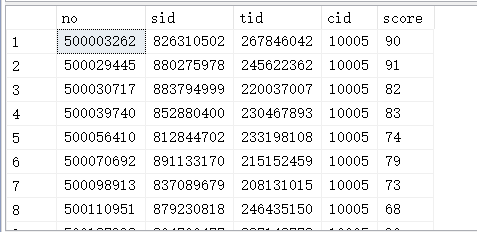
\includegraphics[width=0.9\textwidth]{1.png}
  \end{subfigure}
  \begin{subfigure}{0.2\textwidth}
    \centering
    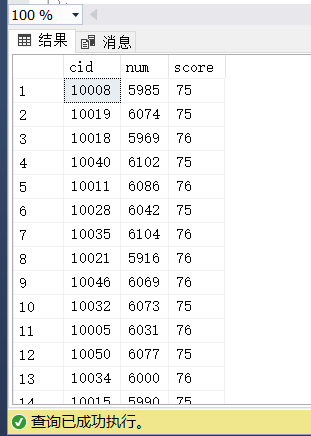
\includegraphics[width=0.9\textwidth]{2.png}
  \end{subfigure}
\end{figure}

  \item 在STUDENTS表中使用SQL语句将姓名为LiMing.的学生的EMAIL改为LM@qq.com。
  \begin{quote}
    \texttt{
      UPDATE STUDENTS SET email = 'LM@qq.com' WHERE sname = 'LIMING';\\
    }
  \end{quote}
  \item 在TEACHERS表中使用SQL语句将所有教师的工资翻倍。
  \begin{quote}
    \texttt{
      UPDATE TEACHERS SET salary = salary*2;\\
    }
  \end{quote}


  \begin{figure}[htb]
    \centering
    \begin{subfigure}{0.4\textwidth}
      \centering
      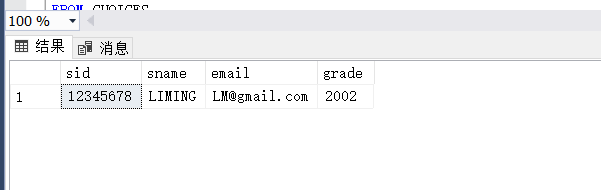
\includegraphics[width=0.9\textwidth]{3.png}
    \end{subfigure}
    \begin{subfigure}{0.4\textwidth}
      \centering
      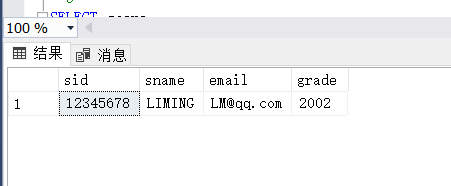
\includegraphics[width=0.9\textwidth]{4.png}
    \end{subfigure}
  \end{figure}
  

  \item 将姓名为waqcj的学生的课程C++的成绩加10分。
  \begin{quote}
    \texttt{
      UPDATE CHOICES SET score = score +10
WHERE sid in (
    SELECT sid
    FROM STUDENTS
    WHERE sname = 'waqcj'
    )AND cid =(
        SELECT cid
        FROM COURSES
        WHERE cname = 'C++'
    );\\
    }
  \end{quote}


  \item 在STUDENTS表中使用SQL语句删除姓名为LiMing的学生信息。
  \begin{quote}
    \texttt{
      DELETE FROM STUDENTS
WHERE sname='LiMing';\\
    }
  \end{quote}


  \begin{figure}[htb]
    \centering
    \begin{subfigure}{0.4\textwidth}
      \centering
      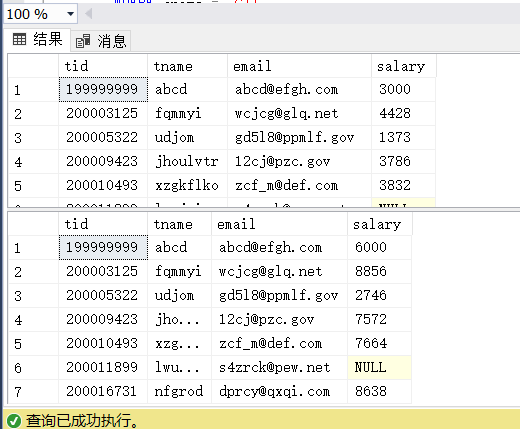
\includegraphics[width=0.9\textwidth]{5.png}
    \end{subfigure}
    \begin{subfigure}{0.4\textwidth}
      \centering
      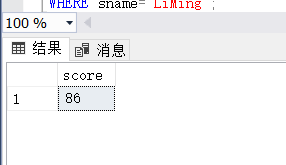
\includegraphics[width=0.9\textwidth]{6.png}
    \end{subfigure}
  \end{figure}
  

  \item 删除所有选修课程C的选课记录。
  \begin{quote}
    \texttt{
DELETE FROM CHOICES
WHERE cid =(
    SELECT cid
    FROM COURSES
    WHERE cname = 'C'
    );\\
    }
  \end{quote}
  \item 对COURSES表做删去时间>80的元组的操作,讨论该删除操作所受到的约束。  
  \begin{quote}
    \texttt{
      DELETE COURSES WHERE hour >= 80;\\
    }
  \end{quote}

  \begin{figure}[htb]
    \centering
    \begin{subfigure}{0.4\textwidth}
      \centering
      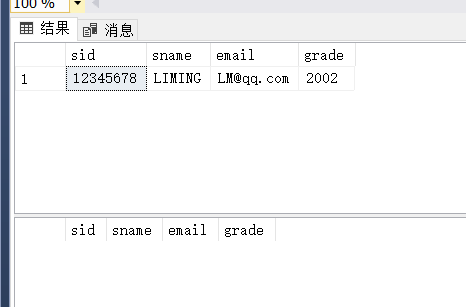
\includegraphics[width=0.9\textwidth]{7.png}
    \end{subfigure}
    \begin{subfigure}{0.4\textwidth}
      \centering
      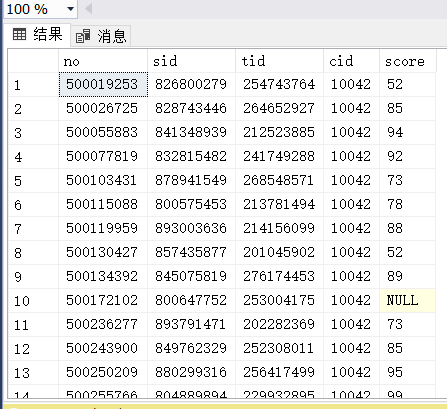
\includegraphics[width=0.9\textwidth]{8.png}
    \end{subfigure}
  \end{figure}
  
\end{enumerate}

\section{实验3.2、视图操作}

\begin{enumerate}
\item	建立薪水大于3000的教师的视图t\_view,并要求进行修改和插入操作时仍需保证该视图只有薪水大于3000的教师信息。
\begin{quote}
  \texttt{
    CREATE VIEW t\_view
AS
    SELECT *
    FROM TEACHERS
    WHERE salary > 3000
    WITH CHECK OPTION;\\
  }
\end{quote}
\item	在视图t\_view中查询邮件地址为xibl@izd.edu的教师的相关信息。
\begin{quote}
  \texttt{
    SELECT *
FROM t\_view
WHERE email = 'xibl@izd.edu';\\
  }
\end{quote}

\begin{figure}[htb]
  \centering
  \begin{subfigure}{0.4\textwidth}
    \centering
    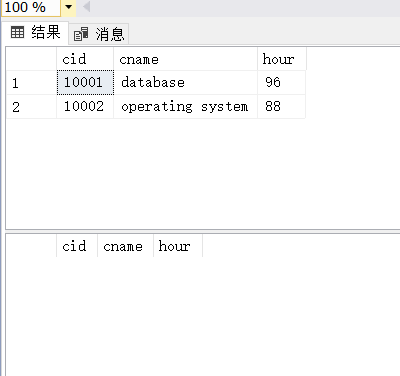
\includegraphics[width=0.9\textwidth]{9.png}
  \end{subfigure}
  \begin{subfigure}{0.4\textwidth}
    \centering
    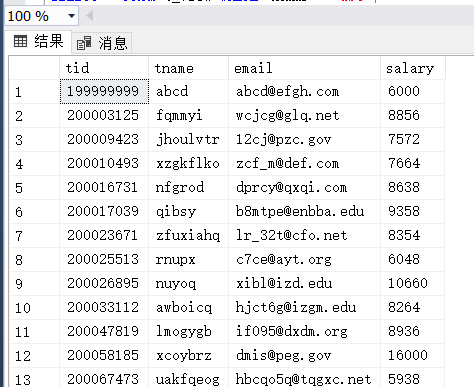
\includegraphics[width=0.9\textwidth]{10.png}
  \end{subfigure}
\end{figure}

\item	向视图t\_view中插入一个新的教师记录,其中教师编号为199999998,姓名为abc,邮件地址为abc@def.com,薪水为5000。
\begin{quote}
  \texttt{
    INSERT INTO t\_view
VALUES ('199999998','abc','abc@def.com',5000);\\
  }
\end{quote}
\item	在视图t\_view中将编号为200010493的教师的薪水改为6000。
\begin{figure}[htb]
  \centering
  \begin{subfigure}{0.4\textwidth}
    \centering
    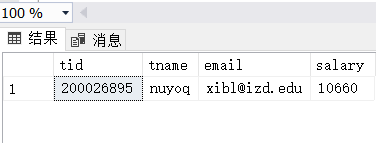
\includegraphics[width=0.9\textwidth]{11.png}
  \end{subfigure}
  \begin{subfigure}{0.4\textwidth}
    \centering
    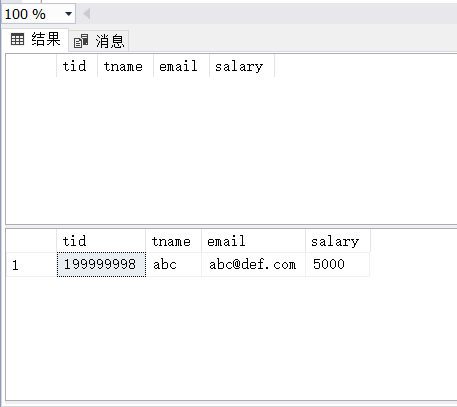
\includegraphics[width=0.9\textwidth]{12.png}
  \end{subfigure}
\end{figure}
\begin{quote}
  \texttt{
UPDATE t\_view SET salary = 6000
WHERE tid = '200010493';\\
  }
\end{quote}

\item	删除视图t\_view。
\begin{quote}
  \texttt{
    DROP VIEW t\_view;\\
  }
\end{quote}

\begin{figure}[htb]
  \centering
  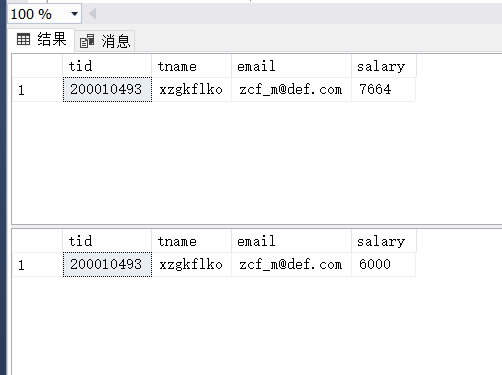
\includegraphics[width=0.4\textwidth]{13.png}
\end{figure}
\end{enumerate}

\section{实验3.3、用户标识与鉴别}

\begin{enumerate}
  \item	在SSMS中,设置SQL Server的安全认证模式。
  \begin{figure}[htb]
    \centering
    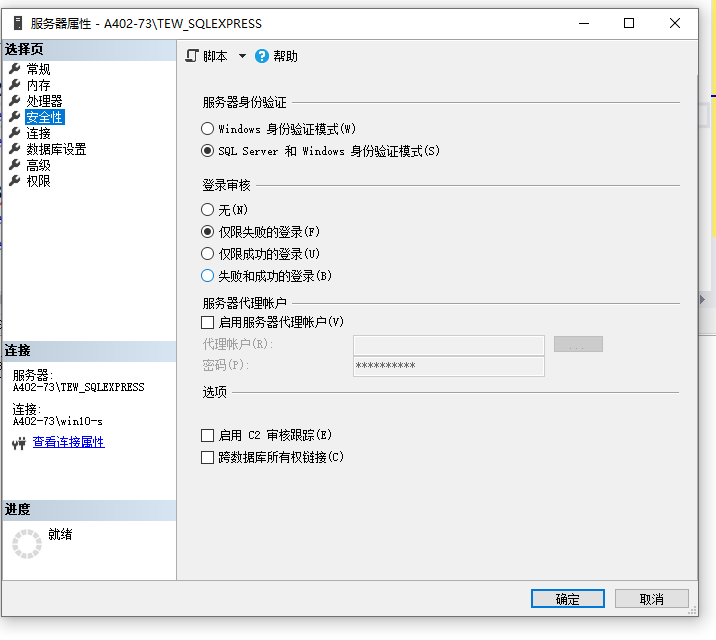
\includegraphics[width=0.4\textwidth]{login.png}
  \end{figure}
  \item	在SSMS中建立一个名为“张三”的登陆用户、School数据库用户。
  \begin{quote}
    \texttt{
      exec sp\_addlogin '张三','Aa[]12345678','School';\\
exec sp\_adduser  '张三';
    }
  \end{quote}
  \item	在SSMS中取消“张三”这个用户。
  \begin{quote}
    \texttt{
exec sp\_dropuser  '张三';
    }
  \end{quote}
\end{enumerate}

\section{实验3.4、自主存取控制}

\begin{enumerate}
  \item	在SSMS中建立一个名为“张三”的登陆用户、School数据库的用户。参见实验3.3的试验步骤(2)
  \begin{quote}
    \texttt{
      exec sp\_addlogin '张三','Aa[]12345678','School';\\
exec sp\_adduser  '张三';\\
    }
  \end{quote}
  \item	使用查询验证“张三”这个用户名是否具有对学生表的SELECT权限。
  \begin{quote}
    \texttt{
EXECUTE AS USER ='张三';\\
SELECT  * FROM  STUDENTS;\\
    }
  \end{quote}

  \begin{figure}[htb]
    \centering
    \begin{subfigure}{0.4\textwidth}
      \centering
      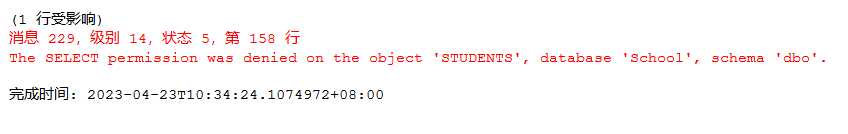
\includegraphics[width=0.9\textwidth]{14.png}
    \end{subfigure}
    \begin{subfigure}{0.4\textwidth}
      \centering
      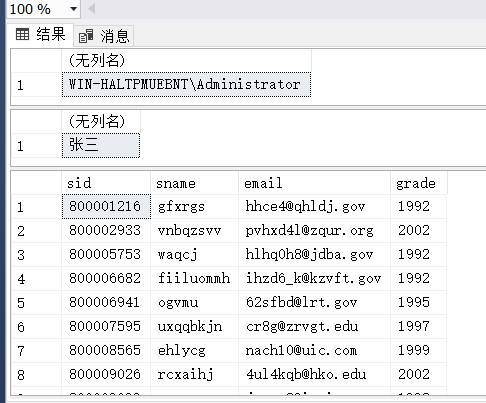
\includegraphics[width=0.9\textwidth]{15.png}
    \end{subfigure}
  \end{figure}

  \item	将School数据库的操作权限赋予数据库用户张三。  
  \begin{quote}
    \texttt{
      REVERT;\\
GRANT ALL PRIVILEGES ON CHOICES TO 张三;\\
GRANT ALL PRIVILEGES ON STUDENTS TO 张三;\\
GRANT ALL PRIVILEGES ON COURSES TO 张三;\\
GRANT ALL PRIVILEGES ON TEACHERS TO 张三;\\
EXECUTE AS USER ='张三';\\
SELECT  * FROM  STUDENTS;\\
    }
  \end{quote}

  \begin{figure}[htb]
    \centering
    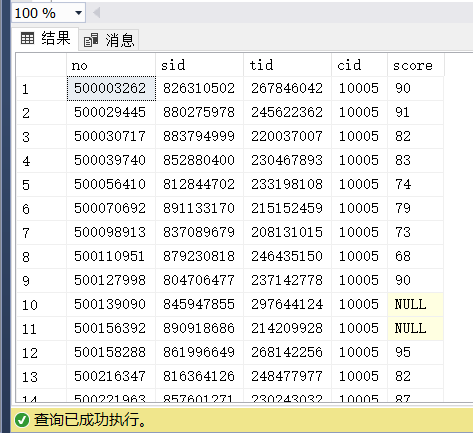
\includegraphics[width=0.4\textwidth]{16.png}
  \end{figure}


\end{enumerate}


\section{实验3.5、视图机制在自主存取控制上的应用}

\begin{enumerate}
\item	在数据库School上创建用户“张三”,具体操作参见实验3.3中的试验步骤(2)。
\begin{quote}
  \texttt{
    exec sp\_addlogin '张三','Aa[]12345678','School';\\ \\
exec sp\_adduser  '张三';\\
  }
\end{quote}
\item	新建查询,用管理员身份登陆数据库。在choices表上创建视图ch\_view,并显示其内容(选课课程号为10005)。
\begin{quote}
  \texttt{
    CREATE VIEW ch\_view
AS
    SELECT * FROM CHOICES
    WHERE cid = '10005';\\
  }
  SELECT * FROM ch\_view;\\
\end{quote}


\item	在视图ch\_view上给用户张三赋予INSERT的权限。
\begin{quote}
  \texttt{
    GRANT INSERT ON ch\_view TO 张三;\\
  }
\end{quote}
\item	将视图ch\_view上score列的权限赋予用户张三。
\begin{quote}
  \texttt{
    GRANT ALL PRIVILEGES ON ch\_view(score) TO 张三;\\
EXECUTE AS USER = '张三';\\
SELECT score FROM ch\_view;\\
  }
\end{quote}
\item	以用户张三登陆查询分析器,对ch\_view进行查询操作。
\begin{quote}
  \texttt{
    REVERT ;\\
GRANT ALL PRIVILEGES ON ch\_view TO 张三;\\
EXECUTE AS USER = '张三';\\
SELECT * FROM ch\_view;\\
  }
\end{quote}
\item	以用户张三登陆查询分析器, 对no为500127998的学生的成绩进行修改,改为90分。
\begin{quote}
  \texttt{
    EXECUTE AS USER = '张三';\\
UPDATE ch\_view SET  score=90
WHERE no = '500127998';\\
  }
\end{quote}
\begin{figure}[htb]
  \centering
  \begin{subfigure}{0.4\textwidth}
    \centering
    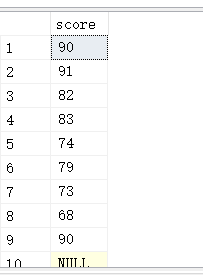
\includegraphics[width=0.9\textwidth]{17.png}
  \end{subfigure}
  \begin{subfigure}{0.4\textwidth}
    \centering
    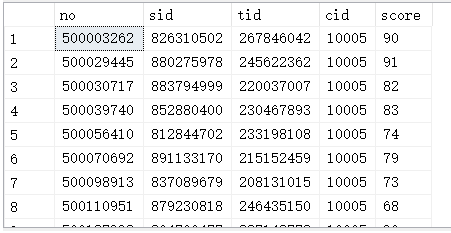
\includegraphics[width=0.9\textwidth]{18.png}
  \end{subfigure}
\end{figure}
\item	收回对用户张三对视图ch\_view查询权限的授权
\begin{quote}
  \texttt{
    REVERT;\\
REVOKE SELECT ON ch\_view TO 张三;\\
EXECUTE AS USER = '张三';\\
  }
\end{quote}
\begin{figure}[htb]
  \centering
  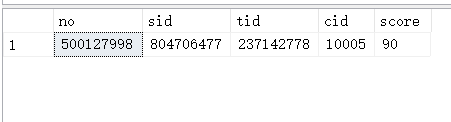
\includegraphics[width=0.4\textwidth]{19.png}
\end{figure}
\end{enumerate}

\section{实验总结}

本次实验主要是对数据库的用户标识与鉴别、自主存取控制、视图机制在自主存取控制上的应用进行了实验,通过实验,我们对数据库的用户标识与鉴别、自主存取控制、视图机制在自主存取控制上的应用有了更深的了解。

\end{spacing}

\end{document}